\input{"./2ProjectSetup".tex}%
\input{"\DenKrAllMainRootDirPATH/2includes/packages/preamble_pre".tex}%
\documentclass[tikz,fontsize=11pt,class=scrbook]{standalone}% I.e. the content from \input{"\DenKrLayoutMainRootDir/2layout/tikz_standalone/preamble_1_class".tex}%
\usepackage{pgfgantt}%
\input{"\DenKrInternalLayoutRootDir/tikz_standalone/1TikzStandalonePicIncludeThis".tex}%
\DenKrTikzStandalonePre%
%
%
%
%
%
% - Decent Default Values
\colorlet{complete}{OliveGreen!75}
\colorlet{pending}{Maroon}
\definecolor{groupblue}{RGB}{51,102,254}
\colorlet{groupblue}{groupblue!70!black}
%
% - Some other Settings
\definecolor{barblue}{RGB}{153,204,254}
\definecolor{linkred}{RGB}{165,0,33}
\setganttlinklabel{s-s}{START-TO-START}
\setganttlinklabel{f-s}{FINISH-TO-START}
\setganttlinklabel{f-f}{FINISH-TO-FINISH}
%
% - Setting-up
% \definecolor{complete}{named}{blue}
\colorlet{pending}{Maroon!80!blue!80!white}
%
%
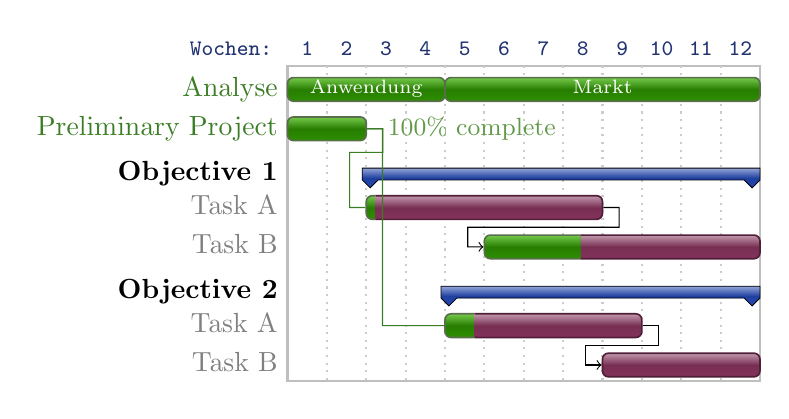
\begin{tikzpicture}[
	scale = 1.0,% Could be the Macro \tikzpicturescale. See in makros.tex
	% (Is supposed to be handed over)(Be mindful of the possibilities for handing over;
	% standalone mode=tex vs mode=buildnew)
	auto,
	node distance=\nodedistance
]
%
\tikzstyle{default_bar}=[
    fill=complete,
    top color=complete!70!white,
    bottom color=complete!80!black,
    middle color=complete!70!black,
    rounded corners=0.5ex,
    draw=complete!60!black,
    line width=0.6pt
]
\tikzstyle{default_bar_incomplete}=[
    fill=pending,
    top color=pending!50!white,
    bottom color=pending,
    middle color=pending!90!black,
    draw=pending!60!black,
    line width=0.6pt
]
\tikzstyle{default_group}=[
    fill=groupblue,
    top color=groupblue!50!white,
    bottom color=groupblue,
    middle color=groupblue!90!black,
    draw=black,
    line width=0.3pt
]
\tikzstyle{default_link}=[
    % -latex,
    -to,
    line width=0.4pt, draw=black
]
%
\begin{ganttchart}[
    canvas/.append style={fill=none, draw=black!25, line width=.75pt},
    y unit title=0.4cm,
    y unit chart=0.5cm,
    % vgrid,
    % hgrid style/.style={draw=black!5, line width=.75pt},
    vgrid={*1{draw=black!20, line width=.75pt, dotted}},
    % today=7,
    % today rule/.style={
    % draw=black!64,
    % dash pattern=on 3.5pt off 4.5pt,
    % line width=1.5pt
    % },
    today label font=\small\bfseries,
    % time slot format=isodate-yearmonth,
    % time slot unit=month,
    % title/.append style={draw=none, fill=RoyalBlue!50!black},
    % title label font=\sffamily\bfseries\color{white},
    % title label node/.append style={below=-1.6ex},
    % title left shift=.05,
    % title right shift=-.05,
    title height=1,
    %
    title/.style={draw=none, fill=none},
    title label font=\ttfamily\footnotesize\color{RoyalBlue!50!black},
    % title label node/.append style={below=7pt},
    include title in canvas=false,
    %
    bar/.append style={default_bar},
    bar incomplete/.append style={default_bar_incomplete},
    bar height=.6,
    bar label font=\normalsize\color{black!50},
    bar inline label node/.style={font={\scriptsize\color{white}}},
    group/.append style={default_group},
    group right shift=0,
    group top shift=.6,
    group height=.3,
    group peaks height=.2,
    %
    link/.style={default_link},
    % link label font=\scriptsize\bfseries,
    % link label node/.append style={below left=-2pt and 0pt},
]{1}{12}
%
%
%
\gantttitle[
    % title label node/.append style={below left=7pt and -3pt}
    title label node/.append style={left=0pt and 0.2em}
]{Wochen:}{0}
\gantttitlelist{1,...,12}{1} \\
%
\ganttset{progress label text={}}

\ganttbar[bar/.style={},
    bar label font=\normalsize\color{OliveGreen},
]{Analyse}{1}{1}
\ganttbar[
    inline,
    % bar progress label font=\small\color{OliveGreen!75},
    % bar progress label node/.append style={right=4pt},
]{Anwendung}{1}{4}
\ganttbar[
    inline,
    progress=100,
    % bar progress label font=\small\color{OliveGreen!75},
    % bar progress label node/.append style={right=4pt},
]{Markt}{5}{12} \\
%
\ganttset{progress label text={\pgfmathprintnumber[precision=0, verbatim]{#1}\% complete}}

\ganttbar[
    progress=100,
    bar progress label font=\small\color{OliveGreen!75},
    bar progress label node/.append style={right=4pt},
    bar label font=\normalsize\color{OliveGreen},
    name=pp
]{Preliminary Project}{1}{2} \\

\ganttset{progress label text={}}

\ganttgroup{Objective 1}{3}{12} \\
\ganttbar[progress=4, name=T1A]{Task A}{3}{8} \\
% \ganttlinkedbar[progress=35, name=T1B]{Task B}{6}{12} \\
\ganttbar[progress=35, name=T1B]{Task B}{6}{12} \\
\ganttlink{T1A}{T1B}

\ganttgroup{Objective 2}{5}{12} \\
\ganttbar[progress=15, name=T2A]{Task A}{5}{09} \\
\ganttlinkedbar[progress=0]{Task B}{9}{12}

\ganttset{link/.style={OliveGreen}}
\ganttlink[link mid=.3]{pp}{T1A}
% \ganttlink[link tolerance=10.1 ,link mid=.1, link bulge=0.7]{pp}{T2A}
\ganttlink[link mid=.2]{pp}{T2A}
%
%
%
\end{ganttchart}
%
\end{tikzpicture}%
%
%
\DenKrTikzStandalonePost%